\chapter{代数拓扑}
    \section{Brouwer不动点定理与Sperner引理}
    我们首先叙述 Brouwer不动点定理与Sperner引理:
    \begin{theorem}[Brouwer不动点定理]
        设 $f$ 是 $n$ 维闭球 $B^n$ 到自身的连续映射, 则 $f$ 必有不动点.
    \end{theorem}
    \begin{lemma}[Sperner引理]
        设 $K=[v_0,\dots,v_n]$ 是 $n$ 维单纯形, 考虑其三角剖分 $T$, 将 $T$ 的顶点 $(n+1)$ 染色, 即定义 $\lambda:V(T)\rightarrow\{0,\dots,n\}$, 且满足对任意指标子集
        $\{i_0,\dots,i_k\}\subseteq\{0,\dots,n\}$, $\lambda$ 在 $[v_{i_0},\dots,v_{i_k}]$ 上的限制的值域包含于 $\{i_0,\dots,i_k\}$. 则一定存在 $u_0,\dots,u_n\in V(T)$, 
        使得 $[u_0,\dots,u_n]$ 是三角剖分 $T$ 的单形, 且 $\lambda(u_i)$ 互不相同.
        \begin{figure}[hbtp]
            \centering
            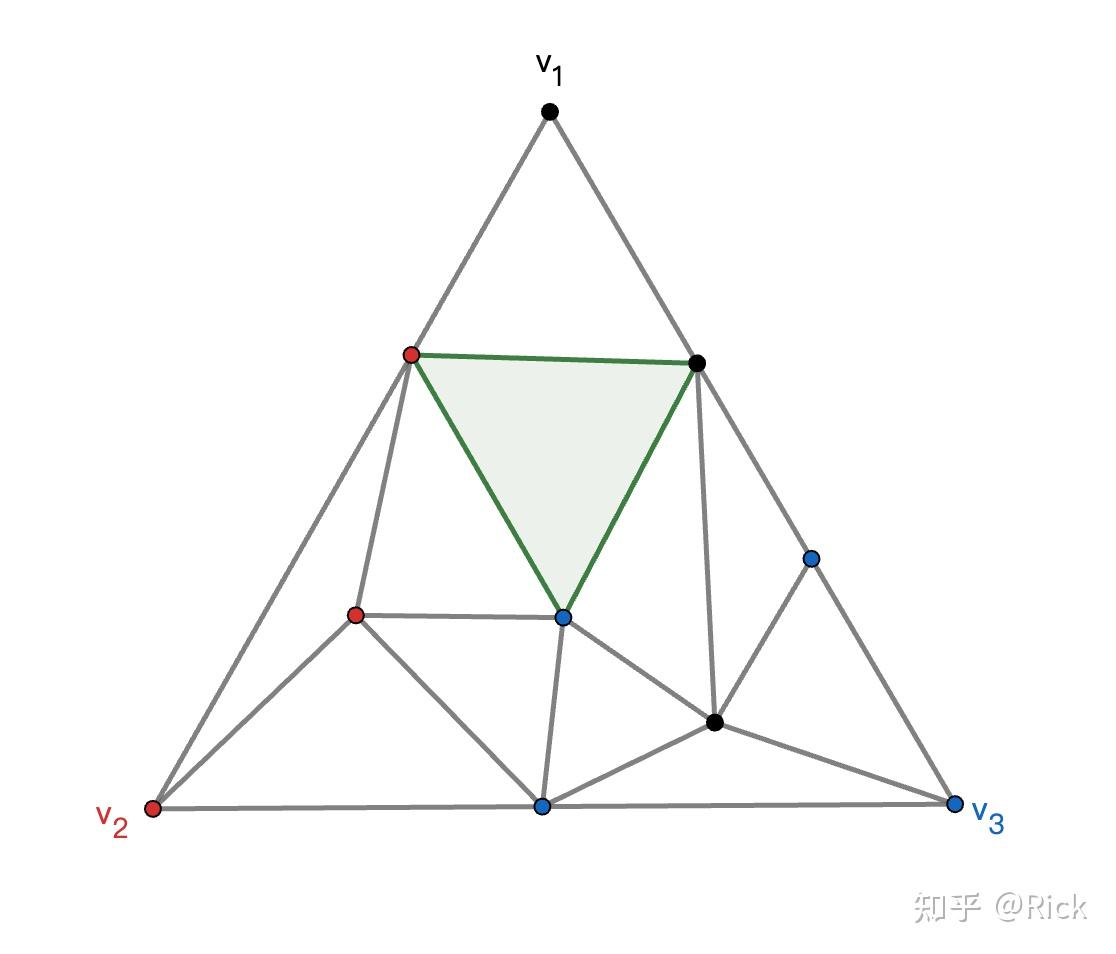
\includegraphics[scale=0.2]{Figures/SpernerLemma.jpg}
            \caption[SpernerLemma]{Sperner引理示意图}
        \end{figure}
    \end{lemma}

    它们一个是拓扑的定理, 一个是组合的定理, 看似没有联系, 但实际上我们能证明它们是等价的: 
    \begin{proof}[{\bf 等价性的证明}]
        由于 $B^n\cong K$, 我们将 Brouwer不动点定理的叙述改为 $K$ 到自身的连续映射 $f$ 必有不动点.

        $1^{\circ}$:Sperner引理 $\Rightarrow$ Brouwer不动点定理
        
        设 $K = [v_0,\dots,v_n]$ 是 $n$ 维单形, 对 $\forall x\in K$, $x=\sum_i\alpha_iv_i,\,\alpha_i\geqslant0,\,\sum_i\alpha_i=1$. 设 $f(x) = \sum_i\beta_iv_i$, 定义染色映射 
        $\lambda(x)$ 为使得 $\alpha_i\geqslant\beta_i$ 且 $\alpha_i\neq0$ 的最小下标 $i$. 我们首先观察到在任意集合 $\{i_0,\dots,i_k\}\subseteq\{0,\dots,n\}$ 中, 
        对 $\forall x\in[v_{i_0},\dots,v_{i_k}]$, $x$ 的坐标 $\alpha$ 满足 $\alpha_i=0,\,i\notin\{i_0,\dots,i_k\}$, 因此 $\lambda(x)$ 只可能在 $\{i_0,\dots,i_k\}$ 中取值.

        固定染色 $\lambda$, 取重心重分 $K^0,K^1,\dots$, 则在每一个 $K^j$ 中 $\lambda$ 均满足引理条件, 于是存在异色单形 $\Delta^j=[u^j_0,\dots,u^j_n]$, 不妨设 $\lambda(u^j_i)=i$.
        因为 $K$ 是紧集, 因此 $\{u^j_0\}_j$ 存在收敛子列, 不妨设就为序列本身, 由重心重分的性质知 $\Delta^j$ 的直径趋于零, 因此对所有 $i$, $\{u^j_i\}_j$ 均收敛于同一点 $u$, 即 
        $u=\lim\limits_{j\rightarrow\infty}u^j_i,\,\forall\,i=0,\dots,n$. 由染色的定义知 $u^j_i$ 的 $v_i$ 坐标不等于零且大于等于 $f(u^j_i)$ 的, 
        根据极限的保号性知 $u$ 的所有坐标 $\alpha_i$ 大于等于 $f(u)$ 对应的坐标 $\beta_i$, 但因为 $\sum_i\alpha_i = \sum_i\beta_i = 1$, 所以 $\alpha_i=\beta_i$, 因此 $u = f(u)$ 是 $f$ 的不动点.

        $2^{\circ}$:Sperner引理 $\Leftarrow$ Brouwer不动点定理
        
        设 $K = [v_0,\dots,v_n]$ 是 $n$ 维单形, $\lambda$ 为满足引理要求的染色, $T$ 是 $K$ 的一个三角剖分, 则可以定义单纯映射 $f:K\rightarrow K$ 如下: 对 $\forall x\in V(T)$, 
        定义 $f(x) = v_{\lambda(x)}$, 若 $x = \sum_{i=0}^{k}\alpha_ix_i$, 其中 $[x_0,\dots,x_k]$ 为 $T$ 的 $k$ 维单形, 定义 $f(x) = \sum_{i=0}^{k}\alpha_iv_{\lambda(x_i)}$.

        若 $T$ 中没有 $n$ 维异色单形, 则 $f$ 的像集包含于 $\partial K$ 中, 且对于每个 $(n-1)$ 维面 $[v_0,\dots,\hat{v_i},\dots,v_n]$ 均有 $f([v_0,\dots,\hat{v_i},\dots,v_n])\subset[v_0,\dots,\hat{v_i},\dots,v_n]$.
        不妨设 $\sum_{i=0}^{n}v_i = 0$, 即 $K$ 的重心是原点. 定义 $g:\partial K\rightarrow \partial K$, $g(x)$ 为射线 $xO$ 与 $\partial K$ 的另一个交点, 类比对径映射. 则 $g([v_0,\dots,\hat{v_i},\dots,v_n])\cap[v_0,\dots,\hat{v_i},\dots,v_n]=\emptyset$
        则 $g\circ f$ 是 $K$ 到自身的连续映射, 但没有不动点, 与Brouwer不动点定理矛盾.
    \end{proof}
    
    现在我们回到Sperner引理本身的证明
    \begin{proof}
        对维数 $n$ 做归纳, 我们证明对任意维数异色单形的个数均为奇数.

        当 $n=1$ 时, $K = [v_0,v_1]$ 可看做闭区间 $[0,1]$, 设 $v_0=x_0<x_1<\cdots<x_m=v_1$ 是剖分 $T$ 中的点, 则 $\#\verb|异色单形| = \#\left\{i\,\big|\,\lambda(x_{i-1})\neq\lambda(x_i)\right\}$. 而
        \begin{equation*}
            1 = \lambda(v_1)-\lambda(v_0) = \sum_{i=1}^{m}\lambda(x_i)-\lambda(x_{i-1}) = \sum_{\lambda(x_{i-1})\neq\lambda(x_i)}\lambda(x_i)-\lambda(x_{i-1})
        \end{equation*} 
        因此 $\#\verb|异色单形|$ 是奇数. 

        假设维数为 $n-1$ 时命题成立, 我们称 $T$ 中的 $(n-1)$ 维单形 $[x_0,\dots,x_{n-1}]$ 为一个好单形, 若 $\{\lambda(x_0),\dots,\lambda(x_{n-1})\} = \{0,\dots,n-1\}$. 对 $T$ 中的  $n$ 维单形
        $\Delta_n=[u_0,\dots,u_n]$, 令 $c(\Delta_n)$ 为 $\Delta_n$ 中好单形的个数, 记 $S=\{\lambda(u_0),\dots,\lambda(u_n)\}$, 则
        \begin{equation*}
            c(\Delta_n)= \left\{
            \begin{aligned}
                0,\; &\{0,\dots,n-1\}\nsubseteq S \\
                2,\; &\{0,\dots,n-1\} = S \\
                1,\; &\{0,\dots,n\} = S  
            \end{aligned}\right. ,
        \end{equation*}
        于是异色单形个数的奇偶性与 $\sum\limits_{\Delta_n\subset T}c(\Delta_n)$ 的奇偶性相同. 而当好单形在 $\overset{\circ}{K}$ 内时, 它是两个 $n$ 单形的公共面; 当好单形在 $\partial K$ 上时, 它仅为一个 $n$ 单形的面.
        因此异色单形个数的奇偶性与 $\partial K$ 上好单形的个数的奇偶性相同, 根据条件好单形仅在 $[v_0,\dots,v_{n-1}]$ 中出现, 由归纳假设知 $[v_0,\dots,v_{n-1}]$ 中好单形有奇数个, 命题成立.
    \end{proof}

    \section[Invariance of domain]{区域不变性定理(Invariance of domain)}
        该定理也是拓扑中的重要定理, 有人说它是欧式空间的内蕴性质, 用它可以区分不同维数的欧式空间.
        \begin{theorem}
            设 $U$ 为 $\mathbb{R}^n$ 中的开子集, $f:U\rightarrow\mathbb{R}^n$ 为连续单射, 则 $f(U)$ 为 $\mathbb{R}^n$ 的开子集且 $f$ 为开映射, 即 $f$ 为 $U$ 到 $f(U)$ 的同胚.
        \end{theorem}

    \section[Poincar\'e Lemma]{Poincar\'e Lemma 的另一种表述形式}
        \begin{lemma}[d-Poincar\'e lemma]
            若整体有 $\md\omega = 0$, 则方程 $\md\eta=\omega$ 局部有解, 即在每点处存在邻域使得方程有解.
        \end{lemma}
        \begin{lemma}[$\overline{\partial}$-Poincar\'e lemma]
            若整体有 $\overline{\partial}\omega = 0$, 则方程 $\overline{\partial}\eta=\omega$ 局部有解, 即在每点处存在邻域使得方程有解.
        \end{lemma}
        \begin{remark}
            因此若整体有 $\md\omega = 0$, 但方程 $\md\eta=\omega$ 在整体上没有解, 这就表明空间本身限制的整体解的存在性, 也就是说我们检测到一个拓扑上的障碍.
        \end{remark}

    \section[Excision Theorem in Signular Homology]{切除定理(Excision Theorem)}
        \begin{theorem}[切除定理表述1]\label{thm:excision-1}
            设 $Z\subset A\subset X$ 满足 $\overline{Z}\subset A^{\circ}$, 则空间偶的嵌入 $(X-Z,A-Z)\hookrightarrow(X,A)$ 诱导了相对同调群之间的同构:
            \begin{equation*}
                H_n(X-Z,A-Z)\overset{\cong}{\longrightarrow} H_n(X,A),\quad n\geq0.
            \end{equation*}
        \end{theorem}
        这个定理有一个等价的表述:
        \begin{theorem}[切除定理表述2]\label{thm:excision-2}
            设 $A,B\subset X$ 且满足 $A^{\circ}\cup B^{\circ}=X$, 则空间偶的嵌入 $(B,A\cap B)\hookrightarrow(X,A)$ 诱导了相对同调群之间的同构:
            \begin{equation*}
                H_n(B,A\cap B)\overset{\cong}{\longrightarrow} H_n(X,A),\quad n\geq0.
            \end{equation*}
        \end{theorem}
        \begin{remark}
            两种表述靠 $B=X-Z\;(Z=X-B)$ 相互转化.
        \end{remark}

        为了证明这个定理, 我们需要先证明同调的“局部性”({\bf locality principal}).

        设 $X$ 是一个拓扑空间, 我们称 $X$ 的子集族 $\mathfrak{U}=\{U_j\}_{j\in J}$ 是一个覆盖, 若 $\{U_j^{\circ}\}_{j\in J}$ 构成一个开覆盖(注意 $U_j$ 本身不必是开集).

        \begin{definition}[{\bf$\mathfrak{U}$-small chains}]\hfill
            \begin{itemize}
                \item 一个 $n$-单形 $\sigma:\Delta^n\rightarrow X$ 被称为 $\mathfrak{U}$-small 的, 若 ${\rm Im}\,\sigma$ 在某个 $U_j$ 中.
                \item 一个 $n$-复形 $c=\sum_i{n_i\sigma_i}$ 被称为 $\mathfrak{U}$-small 的, 若每个 $\sigma_i$ 都是 $\mathfrak{U}$-small 的.
                \item 所有 $\mathfrak{U}$-small 的 $n$-复形构成 $C_n(X)$ 的一个子群, 记为
                \begin{equation*}
                    C^{\mathfrak{U}}_n(X):=\left\{c\in C_n(X)\,\big|\,c \text{ is $\mathfrak{U}$-small}\right\}.
                \end{equation*}
                \item 若 $A\subset X$, 记
                \begin{equation*}
                    C^{\mathfrak{U}}_n(X,A):=\frac{C^{\mathfrak{U}}_n(X)}{C^{\mathfrak{U}}_n(A)}.
                \end{equation*}
            \end{itemize}
        \end{definition}

        若记 $\iota_j:U_j\hookrightarrow X$ 为 $U_j$ 到 $X$ 的嵌入, 那么 $C^{\mathfrak{U}}_n(X)$ 也可以被定义为
        \begin{equation*}
            C^{\mathfrak{U}}_n(X) = {\rm Im}\left(\bigoplus_{j\in J}C_n(U_j)\xrightarrow{\oplus_j (\iota_{j})_*}C_n(X)\right).
        \end{equation*}

        这一概念的关键在于我们可以仅用 $\mathfrak{U}$-small 的链来计算原空间的同调群, 这体现了同调群的局部性.

        \begin{theorem}[{\bf Locality Principle/Small Chain Theorem}]\label{thm:small-chain}
            设 $\mathfrak{U}$ 是 $X$ 的一个覆盖, 则链复形的嵌入映射
            \begin{equation*}
                C^{\mathfrak{U}}_n(X)\subset C_n(X)
            \end{equation*}
            诱导了同调群之间的同构.
        \end{theorem}

        这个定理的证明需要用到重心剖分, 其证明过程有些繁琐, 所以我们跳过该定理的证明, 先看如何用这个定理推导出切除定理.

        \begin{proof}[{\bf Proof of the Excision Axiom using small chains:}]\hfill
            
            我们证明切除定理的表述 $2$, 令 $\mathfrak{U} = \{A,B\}$. 链复形的嵌入映射 $C^{\mathfrak{U}}_n(X)\subset C_n(X)$ 诱导了链复形短正合列之间的一个态射:
            
            \vspace{8pt}
            \begin{tikzcd}
                0 \arrow[r] & C_*(A) \arrow[r] \arrow[d, equal] & C^{\mathfrak{U}}_{*}(X) \arrow[r] \arrow[d] & C^{\mathfrak{U}}_{*}(X)/C_*(A) \arrow[d, dashed] \arrow[r] & 0 \\
                0 \arrow[r] & C_*(A) \arrow[r]                                & C_*(X) \arrow[r]                            & C_*(X)/C_*(A) \arrow[r]                                    & 0
            \end{tikzcd}.
            \vspace{8pt}

            因为中间竖直的映射诱导了同调群之间的同构映射(定理\ref{thm:small-chain}), 由根据短正合引长正合、同调群的自然性、五引理, 
            我们得到右侧竖直映射诱导了同调群的同构, 由此转化为比较 $C_*(B,A\cap B)$ 和 $C^{\mathfrak{U}}_{*}(X)/C_*(A)$.

            注意到
            \begin{gather*}
                C^{\mathfrak{U}}_{*}(X) = C_*(A)+C_*(B)\subset C_*(X), \\
                C_*(A\cap B) = C_*(A)\cap C_*(B).
            \end{gather*}
            因此
            \begin{equation*}
                \frac{C_*(B)}{C_*(A\cap B)}=\frac{C_*(B)}{C_*(A)\cap C_*(B)}\cong\frac{C_*(A)+C_*(B)}{C_*(A)}=\frac{C^{\mathfrak{U}}_{*}(X)}{C_*(A)}.
            \end{equation*}
            中间的同构源自同态基本定理. 

            因此链映射
            \begin{equation*}
                C_*(B,A\cap B)\rightarrow C_*^{\mathfrak{U}}(X)/C_*(A)
            \end{equation*}
            诱导了同调群之间的同构, 原命题成立.
        \end{proof}

        \begin{proof}[{\bf Proof of Locality Principle}]\footnote{证明源自 Hacter 的 Algebraic Topology, 此处是我总结凝练的个人理解.}
            我们需要引入重心重分(或叫重心剖分)这一操作, 需要分几步定义:

            \noindent {\bf Step 1:} 首先定义什么是 $n$-单形 $\Delta^n$ 的重心重分. 为了方便我们使用坐标描述, 
            我们将 $\Delta^n$ 嵌入底空间 $\mathbb{R}^n$, 可用顶点集表示为 $[\ft{v}{0}{n}]$, 
            其中的点可以表示为 $P = \sum_{i=0}^{n}t_iv_i$, $0\leq t_i\leq 1,\;\sum_{t_0}^{n}t_i=1$ 是点 $P$ 的 $n+1$ 个坐标.
            
            我们知道从几何图形上看 $\Delta^n$ 重心重分后是一些更小块的 $n$-单形(带符号),
            但是为了规范叙述重心重分, 我们需要将重分后的对象视为 $LC_n(Y)$ 中的元素, 其中 $Y$ 是某个欧氏空间中的凸集\footnote{这里我很纠结到底用不用书上的记号, 我原本想把每个 $\Delta^n$ 视为 $C_n(\Delta^n)$ 中的元素, 但这样得不到一个链复形, $S$ 和 $T$ 无法定义在一个统一的 $C_*(?)$. 加上线性映射这一条件也是必要的, 否则映射的像就不是规则的图形了.}. 
            也即, 我们把原始的 $\Delta^n$ 视为 $\id:\Delta^n\rightarrow\Delta^n$, 重分后得到 $S\Delta^n\in LC_n(Y)$.

            \noindent$\mathbf{1}^{\circ}$ 锥映射(cone map): 设 $b$ 是 $\mathbb{R}^{n}$ 中的某一个点, 定义以 $b$ 为顶点的锥映射, 写为
            \begin{equation*}
                b:[\ft{v}{0}{n}]\mapsto[b,\ft{v}{0}{n}]
            \end{equation*}
            因此 $b([\ft{v}{0}{n}])$ 中坐标为 $(\ft{t}{0}{n+1})$ 的点是 
            \begin{equation*}
                t_0b+\sum_{t=1}^{n+1}t_iv_i=t_0b+\left(1-t_0\right)\sum_{t=1}^{n+1}\dfrac{t_i}{1-t_0}v_i. 
            \end{equation*}

            \noindent$\mathbf{2}^{\circ}$ 重心重分映射 $S:LC_n(\Delta^n)\rightarrow LC_n(\Delta^n)$. 
            设 $\lambda$ 是一个 $n$-单形, 记 $b_\lambda$ 为 $\lambda$ 的重心, 即所有坐标都取 $\frac{1}{n+1}$ 的点. 我们归纳地定义
            \begin{equation*}
                S\lambda=
                \begin{cases}
                    [\varnothing] &, n = -1;\\
                    b_{\lambda}S(\partial\lambda) &, n \geq 0.
                \end{cases}
            \end{equation*}
            $S$ 在小维数单形上的作用:
            \begin{itemize}
                \item 当 $n=-1$, 即 $\lambda=[\varnothing]$ 时, $S[\varnothing] = [\varnothing]$; 
                \item 当 $n=0$, 即 $\lambda=[w_0]$ 时, $b_\lambda=w_0$, $S[w_0] = w_0S\partial[w_0] = w_0([\varnothing]) = [w_0]$;
                \item  当 $n=1$, 即 $\lambda=[w_0,w_1]$ 时, $S[w_0,w_1] = b_{\lambda}S([w_1]-[w_0]) = [b_{\lambda},w_1]-[b_{\lambda},w_0]$.
            \end{itemize}
            下面归纳地证明 $S$ 是链映射, 即 $S\partial=\partial S$.
            \begin{itemize}
                \item 当 $n=-1,0$ 时, $S = \mathbbm{1}$, 等式显然成立.
                \item 当 $n>0$ 时, 
                \begin{align*}
                    \partial S\lambda &= \partial b_\lambda(S\partial\lambda) \\
                    &= S\partial\lambda-b_\lambda\partial(S\partial\lambda) \qquad \text{因为}\; \partial b_\lambda=\mathbbm{1}-b_\lambda\partial \\
                    &= S\partial\lambda-b_\lambda(S\partial\partial\lambda) \qquad \text{因为归纳假设}\; \partial S(\partial\lambda) = S\partial(\partial\lambda) \\
                    &= S\partial\lambda \qquad \text{因为}\; \partial\partial=0.
                \end{align*}
            \end{itemize}

            \noindent$\mathbf{3}^{\circ}$ $\id$ 和 $S$ 的链同伦 $T:C_n(Y)\rightarrow C_{n+1}(Y)$, 我们归纳地定义
            \begin{equation*}
                T\lambda = 
                \begin{cases}
                    0 &, n = -1; \\
                    b_{\lambda}(\lambda-T\partial\lambda) &, n\geq0.
                \end{cases}
            \end{equation*}
            \begin{center}
                \begin{tikzcd}[column sep=1.8em]
                    \cdots \arrow[r] & LC_{2}(Y) \arrow[r] \arrow[d, "S"] & LC_{1}(Y) \arrow[r] \arrow[d, "S"] \arrow[ld, "T"'] & LC_{0}(Y) \arrow[r] \arrow[d, "S"', "\mathbbm{1}"] \arrow[ld, "T"'] & LC_{-1}(Y) \arrow[r] \arrow[d, "S"', "\mathbbm{1}"] \arrow[ld, "T"', "0"] & 0 \\
                    \cdots \arrow[r] & LC_{2}(Y) \arrow[r]                & LC_{1}(Y) \arrow[r]                                 & LC_{0}(Y) \arrow[r]                                         & LC_{-1}(Y) \arrow[r]                                              & 0
                \end{tikzcd}
            \end{center}
            $T$ 在小维数单形上的作用:
            \begin{itemize}
                \item  当 $n=-1$, 即 $\lambda=[\varnothing]$ 时, $T[\varnothing] = 0$; 
                \item 当 $n=0$, 即 $\lambda=[w_0]$ 时, $b_\lambda=w_0$, $T[w_0] = w_0([w_0]-T\partial[w_0]) = w_0([w_0]) = [w_0.w_0]$;
                \item  当 $n=1$, 即 $\lambda=[w_0,w_1]$ 时, $T[w_0,w_1] = b_{\lambda}\Big([w_0,w_1]-T([w_1]-[w_0])\Big) = [b_{\lambda},w_0,w_1]-[w_1,w_1]+[w_0,w_0]$.
            \end{itemize}
            $T$ 的几何解释如下: 将 $\Delta^n\times I$ 分成若干个 $\Delta^n$, 满足下底 $\Delta^n\times\{0\}$ 仍为一整个 $\Delta^n$(代表 $\id$), 
            上底则成为重心重分后的图形(代表 $S\Delta^n$). $T$ 作用在某个 $\lambda$ 上可能会出现 $[w_0,w_0]$ 这样的元素, 
            对此我们可以将前一个 $w_0$ 视作时间参数 $t=1$ 的点, 后一个视作 $t=0$ 的点, 通过人为增添一个时间维度(即乘以 $I$), 我们能更好地想象 $T$ 的几何动机, 
            $T$ 实际作用的像是前文描述的图形在投影 $\Delta^n\times I\rightarrow\Delta^n$ 下的像.
            \begin{figure}[hbtp]
                \centering
                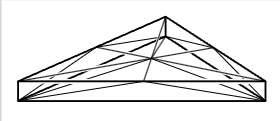
\includegraphics{./Figures/重心重分与恒同的链同论.png}
                \caption{重心重分与恒同的链同论}
                \label{figure:chain_homo_T}
            \end{figure}
            下面归纳地验证 $T$ 是连接 $\id$ 和 $S$ 的链同论, 即 $\partial T+T\partial=\mathbbm{1} - S$:
            \begin{itemize}
                \item 当 $n=-1$ 时, $S = \mathbbm{1}, T=0$, 显然成立.
                \item 当 $n\geq0$ 时, 
                \begin{align*}
                    \partial T\lambda &= \partial b_\lambda(\lambda-T\partial\lambda) \\
                    &= (\lambda-T\partial\lambda) - b_\lambda\partial(\lambda-T\partial\lambda)\qquad\text{因为}\;\partial b_\lambda=\mathbbm{1}-b_\lambda\partial \\
                    &= \lambda-T\partial\lambda - b_\lambda\partial\lambda + b_\lambda\partial T\partial\lambda \\
                    &= \lambda-T\partial\lambda - b_\lambda\partial\lambda + b_\lambda(\partial\lambda - S\partial\lambda - T\partial\partial\lambda)\qquad\text{因为归纳假设} \\
                    &= \lambda-T\partial\lambda - b_\lambda(S\partial\lambda) \\
                    &= \lambda - S\lambda - T\partial\lambda.
                \end{align*}
            \end{itemize}

            \noindent {\bf Step 2:} 对一般的链 $\sigma:\Delta^n\rightarrow X$ 定义重心重分.

            \noindent$\mathbf{1}^\circ$ 定义 $S:C_n(X)\rightarrow C_n(X)$ 为
            \begin{equation*}
                S\sigma=\sigma_\sharp S\Delta^n
            \end{equation*}
            下面的示意图能帮助我们理解 $S$ 的定义.
            \begin{figure}[hbtp]
                \centering
                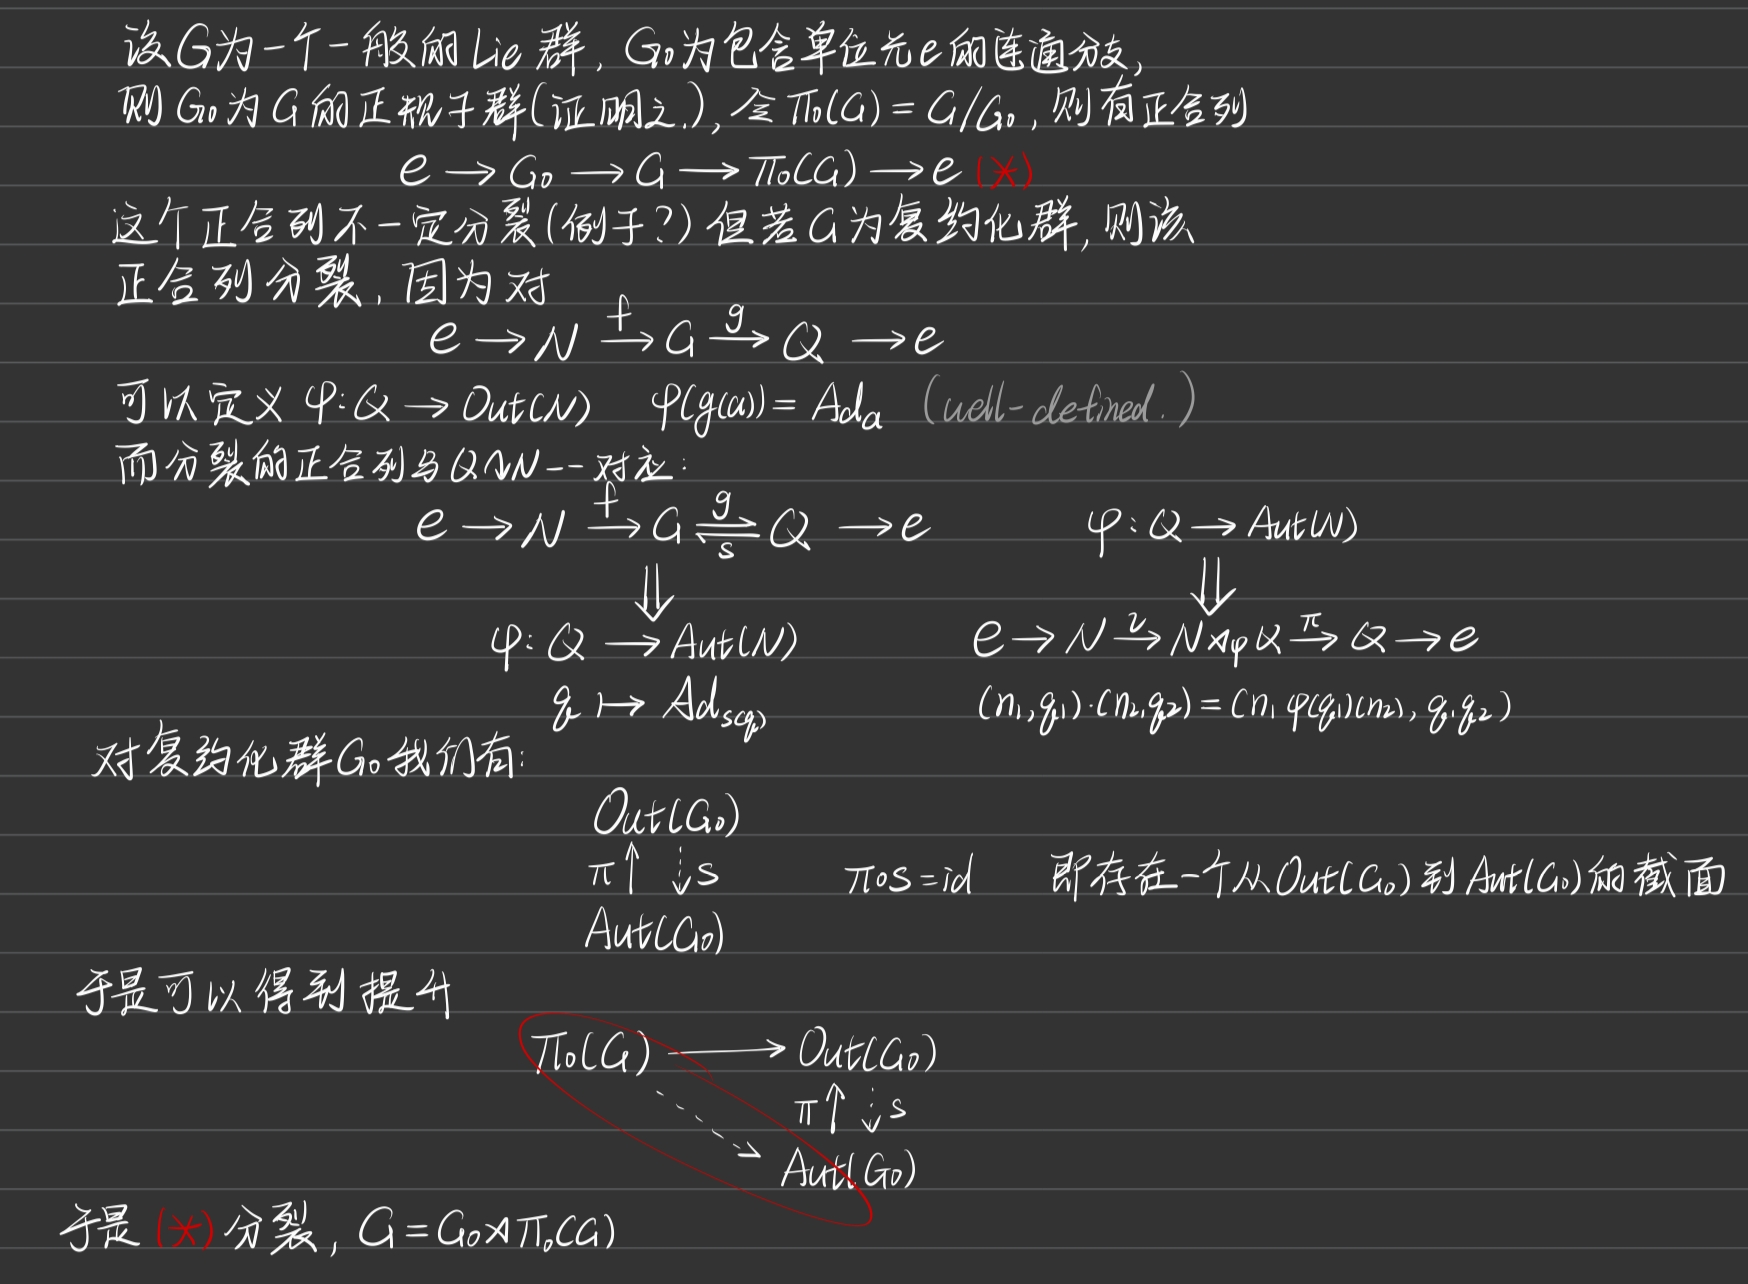
\includegraphics[scale=0.2]{./Figures/20240926-223647.jpg}
                \caption{重心重分与恒同的链同论}
                \label{figure:general_S}
            \end{figure}
            下面验证 $S$ 是一个链映射, 即 $\partial S = S\partial$:
            \begin{align*}
                \partial S\sigma &= \partial\sigma_\sharp S\Delta^n = \sigma_\sharp\partial S\Delta^n = \sigma_\sharp S\partial\Delta^n \\
                &= \sigma_\sharp S\sum_{i=0}^{n}(-1)^i\Delta^n_i \\
                &= \sum_{i=0}^{n}(-1)^i\sigma_\sharp S\Delta^n_i \\
                &= \sum_{i=0}^{n}(-1)^i S(\sigma|_{\Delta^n}) \\
                &= S\left(\sum_{i=0}^{n}(-1)^i \sigma|_{\Delta^n}\right) = S(\partial\sigma).
            \end{align*}
            \noindent$\mathbf{2}^\circ$ 类似地定义 $T:C_n(X)\rightarrow C_{n+1}(X)$ 为
            \begin{equation*}
                T\sigma=\sigma_\sharp T\Delta^n
            \end{equation*}
            下面验证 $T$ 是一个链同伦, 即 $\partial T + T\partial = \mathbbm{1} - S$:
            \begin{align*}
                \partial T\sigma &= \partial\sigma_\sharp T\Delta^n = \sigma_\sharp\partial T\Delta^n \\
                &= \sigma_\sharp(\mathbbm{1}-S - T\partial)\Delta^n \\
                &= \sigma-S\sigma-\sigma_\sharp T\partial\Delta^n\qquad\text{和上面的过程类似} \\
                &= \sigma-S\sigma-T\partial\sigma.
            \end{align*}

            \noindent {\bf Step 3:} 迭代重心重分操作.

            \noindent$\mathbf{1}^\circ$ 可以证明对 $\Delta^n$ 做一次重心重分得到 $(n+1)!$ 个小的 $n$-复形, 这些 $n$-复形的最大直径不超过原复形的 $\frac{n}{n+1}$.
            这个仅依赖于维数的严格小于1的常数是重心重分的一个关键性质. 它保证了只要重分足够多次, 每个 $n$-复形的直径可以任意小.

            现设 $\mathfrak{U}=\{U_{\alpha}\}_{\alpha}$ 是 $X$ 的一个覆盖, 则对单形 $\sigma:\Delta^n\rightarrow X$, $\{\sigma^{-1}U_{\alpha}\}_{\alpha}$ 构成 $\Delta^n$ 的一个开覆盖, 
            因为 $\Delta^n$ 是完备度量空间, 设 $\delta_\sigma$ 是 $\{\sigma^{-1}U_{\alpha}\}_{\alpha}$ 的 Lebesuge 数. 则当 $m$ 充分大时, $S^m\Delta^n$ 中的每个单形的直径都小于 $\delta_\sigma$.
            对一般的链 $\sigma\in C_n(X)$, 记 $m(\sigma)$ 为最小的使得 $S^m\sigma\in C^{\mathfrak{U}}_n(X)$ 的迭代数 $m$.

            连接 $\mathbbm{1}$ 和 $S^m$ 的链同论是 $D_m=\sum\limits_{i=0}^{m-1}TS^i$, 其验证如下:
            \begin{align*}
                \partial D_m + D_m\partial &= \sum_{i=0}^{m-1}\partial TS^i + \sum_{i=0}^{m-1}TS^i\partial \\
                &= \sum_{i=0}^{m-1}(\mathbbm{1} - S - T\partial)S^i + \sum_{i=0}^{m-1}TS^i\partial \\
                &= \sum_{i=0}^{m-1}(\mathbbm{1} - S)S^i - \sum_{i=0}^{m-1}T\partial S^i + \sum_{i=0}^{m-1}TS^i\partial \\
                &= \mathbbm{1} - S^m.
            \end{align*}
           
            对一般的链 $\sigma$, 若定义 $S\sigma = S^{m(\sigma)}\sigma$, 则不能良定义链同论 $D\sigma$, 因为如果定义 $D\sigma = D_{m(\sigma)}\sigma$, 
            公式 $\partial D\sigma+D\partial\sigma = \partial D_{m(\sigma)}\sigma+D_{m(\partial\sigma)}\partial\sigma$, 下指标不全是 $m(\sigma)$. 
             
            因此我们得先定义 $D\sigma := D_{m(\sigma)}\sigma$, 再形式地定义 $\rho:C_n(X)\rightarrow C^{\mathfrak{U}}_n(X)$, 
            \begin{equation*}
                \rho := \mathbbm{1} - \partial D - D\partial
            \end{equation*}
            需要验证 $\rho$ 是链映射, 即 $\partial\rho=\rho\partial$:
            \begin{align*}
                \partial\rho\sigma &= \partial\sigma - \partial\partial D\sigma - \partial D\partial\sigma \\
                &= \partial\sigma - \partial D\partial\sigma \\
                &= \partial\sigma - \partial D\partial\sigma - D\partial\partial\sigma \\
                &= (\mathbbm{1} - \partial D - D\partial)\partial\sigma = \rho\partial\sigma.
            \end{align*}
            由 $\rho$ 的定义易知 $D$ 是 $\mathbbm{1}$ 与 $\rho$ 的链同论.

            最后验证 $\rho$ 确实将 $C_n(\Delta^n)$ 中的元素映到 $C^{\mathfrak{U}}_n(X)$ 中:
            \begin{align*}
                \rho\sigma &= \sigma - \partial D_{m(\sigma)}\sigma - D_{m(\partial\sigma)}\partial\sigma \\
                &= S^{m(\sigma)}\sigma + D_{m(\sigma)}\partial\sigma - D_{m(\partial\sigma)}\partial\sigma \\
                &= S^{m(\sigma)}\sigma + \sum_{m(\partial\sigma) \leq i < m(\sigma)}TS^i\partial\sigma 
            \end{align*}
            因为 $\partial\sigma\subset\sigma$, 所以 $m(\partial\sigma)\leq m(\sigma)$, 由 $m(\sigma)$ 的定义以及 $T$ 保持 $C^{\mathfrak{U}}_n(X)$ 不动,
            等号末项属于 $C^{\mathfrak{U}}_n(X)$, 因此 $\rho$ 就是我们想要的映射.

            \noindent {\bf 总结:} 我们有嵌入映射 $\iota:C^{\mathfrak{U}}_n(X)\hookrightarrow C_n(X)$, 然后我们又定义了 $\rho:C_n(\Delta^n)\rightarrow C^{\mathfrak{U}}_n(X)$, 
            以及 $D:C_n(X)\rightarrow C_{n+1}(X)$, 使得 $\partial D + D\partial = \mathbbm{1} - \rho$. 显然 $\rho\iota = \mathbbm{1}$, 因此 $\rho$ 是 $\iota$ 的同伦逆, 
            也即 $C^{\mathfrak{U}}_n(X)\hookrightarrow C_n(X)$ 诱导了同调群之间的同构.
        \end{proof}

        
        % \begin{tikzcd}
        %     & {H_n(U_i, U_i - x_i)} \arrow[r, "f_*"] \arrow[d, "k_i"] \arrow[ld, "\cong"'] & {H_n(V, V - y)} \arrow[d, "\cong"] \\
        %     {H_n(S^n, S^n - x_i)} & {H_n(S^n, S^n - f^{-1}(y))} \arrow[r, "f_*"] \arrow[l, "p_i"]                & {H_n(S^n, S^n - y)}                \\
        %     & H_n(S^n) \arrow[r, "f_*"] \arrow[u, "j"'] \arrow[lu, "\cong"]                & H_n(S^n) \arrow[u, "\cong"']      
        % \end{tikzcd}
 
        % \begin{tikzcd}[column sep=-1.2em, row sep=1.2em]
        %                                                                    &                                         &                                                           & 0                                        &                               \\
        %     0 \arrow[rd]                                                   &                                         & H_n(X^{n+1}) \arrow[ru]                                   &                                          &                               \\
        %                                                                    & H_n(X^{n}) \arrow[ru] \arrow[rd, "j_n"] &                                                           &                                          &                               \\
        %     {H_{n+1}(X^{n+1},X^n)} \arrow[rr] \arrow[ru, "\partial_{n+1}"] &                                         & {H_n(X^{n},X^{n-1})} \arrow[rd, "\partial_n"'] \arrow[rr] &                                          & {H_{n-1}(X^{n-1},X^{n-2})}    \\
        %                                                                    &                                         &                                                           &  H_{n-1}(X^{n-1}) \arrow[ru, "j_{n-1}"'] &                               \\
        %                                                                    &                                         & 0 \arrow[ru]                                              &                                          &                           
        % \end{tikzcd}

    \section[紧支集上同调]{紧支集上同调\footnote{这一段完全摘抄自\url{https://people.math.wisc.edu/~lmaxim/Topnotes9.pdf}}}
    Let \( X \) be a topological space and \( K \) be a compact subset of \( X \), then
    \begin{align*}
        C_c^i(X) := \bigcup_K C^i(X, X \setminus K) &= \Big\{\varphi : C_i(X) \to \mathbb{Z} \, \big| \, \exists \, \text{compact } K_\varphi \subset X \\
        &\text{ s.t. } \varphi = 0 \text{ on chains in } X \setminus K_\varphi\Big\} \subset C^i(X).
    \end{align*}
    Define \( \delta \varphi(\sigma) := \varphi(\partial\sigma) \), note if \( \varphi \in C_c^i(X) \), then \( \delta \varphi \) is also zero on all chains in \( X \setminus K_\varphi \) and so \( \delta \varphi \in C_c^{i+1}(X) \). Then we get a cochain subcomplex \( C_c^*(X) \).
    \begin{definition}
        $H_c^i(X) := H^i(C_c^*(X))$ is called the cohomology of $X$ with compact support.
    \end{definition}
    
    这个定义和紧支集 de Rham 上同调是一致的.

    \begin{theorem}[紧支集上同调与相对上同调\footnote{有点抽象废话的意思, 能增进我的理解, 但是无法将其与其它更熟悉的概念联系起来.}]
        \( H_{c}^{i}(X) \cong \lim\limits_{K \in I} H^{i}(X, X \setminus K) \) where \( K \) denotes a compact subset of $X$.
    \end{theorem}
    \begin{proof}
        Let \( I = \{ K \subset X \mid K \text{ compact} \} \), 
        and then \( I \) is a directed set since it is partially ordered by inclusion, 
        and the union of two compact sets is also compact. 
        Let \( K \subset L \) be compact subsets of \( X \), 
        then there is a homomorphism \( f_{KL} : H^i(X, X \setminus K) \to H^i(X, X \setminus L) \) induced by inclusion. 
        Note since each element of \( \varinjlim H^i(X, X \setminus K) \) is represented by some cocycle \( \varphi \in C^i(X, X \setminus K) \) for some compact \( K \) with \( [\varphi] \in H_c^i(X) \), 
        and such \( \varphi \) is the zero element in \( \varinjlim H^i(X, X \setminus K) \) iff \( \varphi = \delta \psi \) for some \( \psi \in C^i(X, X \setminus L) \), 
        and so \( [\varphi] = 0 \) in \( H_c^i(X) \). 
        Thus \( H_c^i(X) \cong \varinjlim H^i(X, X \setminus K) \).
    \end{proof}

    \begin{theorem}[紧支集上同调与一点紧化空间的约化上同调]\label{thm:c-cohomology_v.s._reductive_cohomology}
        Let $X^{+} = X \cup \{\infty\}$ be one piont compactification of $X$. Then $H^*_c(X)\cong H^*(X^+,\infty)\cong\tilde{H}^*(X^+)$.
    \end{theorem}
    \begin{proof}
        Consider $U\overset{open}{\hookrightarrow} X \hookleftarrow X\setminus U$, we have a short exact sequence:
        
        \begin{center}
            \begin{tikzcd}[row sep = 0, column sep = 1.8em]
                0 \arrow[r] & \Omega^*_c(U) \arrow[r]   & \Omega^*_c(X) \arrow[r]   & \Omega^*_c(X\setminus U) \arrow[r] & 0 \\
                            & \theta \arrow[r, maps to] & j_*\theta                 &                                    &   \\
                            &                           & \omega \arrow[r, maps to] & \iota^*\omega                      &  
            \end{tikzcd}
        \end{center}
        where $j_*$ means extension by zero, $\iota^*$ is the pull-back of $\iota:X\setminus U\hookrightarrow X$.
        So we can get a long exact sequnce of cohomology with compact support:
        \begin{equation*}
            \cdots\rightarrow H^n_c(U)\rightarrow H^n_c(X)\rightarrow H^n_c(X\setminus U)\rightarrow H^{n+1}_c(U)\rightarrow\cdots
        \end{equation*}
        In case of $X^+ = X\cup\{\infty\}\}$, we get:
        \begin{equation*}
            \cdots\rightarrow H^n_c(X)\rightarrow H^n_c(X^+)\rightarrow H^n_c(\{\infty\})\rightarrow H^{n+1}_c(X)\rightarrow\cdots
        \end{equation*}
        Since both $X^+$ and $\{\infty\}$ are compact, we have
        \begin{equation*}
            \cdots\rightarrow H^n_c(X)\rightarrow H^n(X^+)\rightarrow H^n(\{\infty\})\rightarrow H^{n+1}_c(X)\rightarrow\cdots
        \end{equation*}
        Thus 
        \begin{equation*}
            H^n_c(X)\cong H^n(X^+,\{\infty\})\cong\tilde{H}^n(X^+).
        \end{equation*}
    \end{proof}
    类似的事情对于de Rham上同调也成立.

